\documentclass{amsart}
\usepackage{graphicx}
\graphicspath{{./}}
\usepackage{hyperref}
\usepackage{csvsimple}
\usepackage{longtable}
\usepackage{epigraph}
\title{Zulf Invents Log-V Exponential Models For Human Values}
\author{Zulfikar Moinuddin Ahmed}
\date{\today}
\begin{document}
\maketitle

\section{Log-V Exponential Models}

We are interested in V-shaped linear models for univariate data.  Our interest is not academic or from creative curiosity of arbitrary statistical models.  They arise from observations of Human Nature Value data.  

\section{Log-V Model Idea}

The idea is that univariate data often deviate from exponential distribution in such a way that the mass of the data follow the exponential distribution, but the tail curves upward rather than downward.

Let us consider the measured data $X=(x_1, \dots, x_N)$.  We want to model the data by fitting parameters $\theta = (a_1, b_1, a_2, b_2, x_0)$.  The geometric meaning is that the data comes from the intersection of two lines separated by $x_0$.  

For $x\le x_0$ the data are $y \sim a_1 x + b_1$ and for $x\ge x_0$ the data are from $y \sim a_2 x + b_2$. 

We are interested in the situations where the maximum likelihood fit of the data will yield $a_1 < 0$ and $a_2>0$. 

The above specification is based on observed data rather than purely technical interest in fitting exotic models.

\section{Canonical Log-Likelihood Approach to Fitting Log-V Models}

The log-likelihood of the models is 
\begin{equation}
\ell(X | \theta ) = \sum_{x_j \le x_0} (y_j - a_1 x_j - b_1)^2 + \sum_{x_j \ge x_0} (y_j - a_2 x_j - b_2)^2
\end{equation}

There ought to be many nice ways of fitting this efficiently.  We will not worry about maximal efficiency.  Rather, we will seek an approximate implementation that will yield good maximum-likelihood relative to the more parsimonious linear model.  

The simple linear model has parameters $(a,b)$.  We are introducing three new parameters in addition. 

We want to carefully consider the metrics for goodness of fit.  Obviously log-likelihood will increase with more parameters.  We then need to understand how to quantify comparison of including a penalty for additional parameters.  We don't want a fussy discussion for penalisation and will just use Bayesian Information Criterion.  Thus we will add penalty 
\[
3 \log(N)
\]
when we decide whether to go with the additional parameter.

\section{Expectations}

Since implementing this is some effort, let us consider what we are expecting.  We're going to consider $a_1$ as a Rousseau factor for values and $a_2$ as a Hobbes factor.  

We want to choose between a simple linear model for the entire data.  At the moment $x=(1,\dots,10)$ to be concrete.  So this is not obvious at all how choose the penalisation to produce good models of the data.

\section{Aside:  Good Scientists Do Not Let Accounting Get in the Way}

Classical Statistical Tests are quite good for many issues, and there is a tradition of accounting.  A good scientist does not actually worry all that much about these procedures in the end.  You seem surprised. Well, good scientists don't actually give a damn about any procedures because Nature does not give a fuck about what procedures we pick.  A good scientist will throw out all of statistical theory into the fire if there is a good model that tells us secrets of Nature better that breaks all statistical rules.  This is what happens when you are past studying for exams and so on.  You just don't care about the rules.

\section{Theorising Human Nature From Statistics}

The conflict between Rousseau and Hobbes is in a sense unresolvable in the sense our discovery of exponential law favours Rousseau strongly.  And yet Hobbes cannot be dismissed.  My statistical models of Human Nature provides some new opportunities to understand Human Nature in these poles of Good and Evil.  The savage and aggressive tendencies of Man exist in all of us as well. 

We can consider the equilibrium positions that people arrive, say, on Justifiability of Political Violence as potential for both Good and Evil that are {\em approximately the same in everyone} reaching some comfortable point.  And thus we can see the statistical distributions as a means to understand what all of us are made of realised in a statistical distribution where large numbers of people have chosen their comfortable spots and therefore the latent variable models can estimate the entire Human Moral Animal and Human Nature giving us the measurements of Good and Evil within us all.  And this is an exciting new direction.  Thus when people choose extreme positions on justifiability of political violence, they are not actually different from most of us but have realised some potential in us that we had come not to realise whether by choice, or by habits, or by other means internal to our bodies.  And that allows us to find in latent variable models something about ourselves.  There is clearly much weaker effect of the "Savage Poles" of our Nature than the "Good Poles" since the latter dominate most of Human Race numerically by explicit realisation.  I do not think the "Savage Pole" is actually alien to us either but we do not pursue it with as much passion as some.

This is interesting because I have come across many cynical people in my life who call only the latter "Human Nature" which is quite humorous.  These are Human Nature in a much less important than benevolence, good, cooperative, and other socially positive effects.  


\section{Experiments to Understand the Problem}

There are all sorts of theories out there about model selection, about Akaike Information Criterion or Bayesian Information Criterion.  I have deep skepticism about the claims of these theories.  They are all based on various sorts of unchecked assumptions.  The fact is that in actual situations of data from Nature, we have very little intuition about what these penalties actually measure, and whether they are adequate penalties that will pick any 'true model' at all.  I am a good scientist and do not like statistical theorists talk about 'truth' and 'true model' as though their theories will actually lead to selection of any true model of Nature.  Nature is totally unknown and does not actually behave in such a way that simple arithmetic expressions in penalty terms of any log-likelihood can reveal her secret intentions.  It is a delusion without any limits when statistical theorists sell their snake-oil of the universal form of penalty that will always reveal the secrets of Nature from arbitrary Natural measurements.  Once in a while I do come across such gullible faithful in the Prophets of Akaike and Bayesian Information Criterion.  They always remind me of the "Jesus freaks out in the streets handing out tickets to God" in Elton John's "Tiny Dancer".  Such faith is disturbing for a scientist, truly disturbing.

Let me show you how subtle things are in the world where I live, the world where simple penalties do not give us any comfort that the criteria will pick any 'true model' at all.

Let us go through some elementary issues.  We will denote log-likelihood by $\ell$.  It was a beautiful discovery of Carl Friedrich Gauss, before the likelihood theory became prominent, that univariate regression for $(y,x)$ with data $y=(y_1,\dots, y_N)$ and $x=(x_1, \dots, x_N)$ is obtained by {\em minimizing}

\begin{equation}
F(a,b; y,x) = \sum_{1\le j \le N} (y_j - ax_j - b)^2
\end{equation}
This is the negative of log-likelihood of the univariate linear model.

I always get signs confused if I try to do things quickly.  So let us get the signs straight.

We introduce the notation
\[
\ell_N( x,y |a, b) = - F(a,b | x,y)
\]
The terminology is the 'log-likehood of data given the parameters'.

And now linear regression is {\em maximizing} $\ell_N(x,y|a,b)$ over all possible $a,b\in\mathbf{R}$ which is a calculus exercise in this case.

Suppose we introduce a penalty term to the objective.  The sign is always confusing.  For penalty term $w(x) \ge 0$

\begin{equation}
\ell'_N(x) = \ell_N(x) - w(x)
\end{equation}
The sign here is {\em negative} for the penalty.  This sign causes a lot of problems for me because in actuality one minimizes things in optimisation programs $-\ell_N(x|a,b)+w(x)$
and then we have the positive sign for $w(x)$.

We are interested in some $w(x)$ that will give us the correct {\em model of Nature}.  This is the tricky issue.  We never actually care about sophisticated mathematical issues in the end.  We care to understand how things in Nature work and all our various mathematical chit-chat is supposed to convince both us and our various audience that we have some confidence that all this mathematical infrastructure will reveal the secrets of Nature.  This is a con game.  We are in fact selling snake-oil when we give this impression.  This impression is deceptive.  We have no idea if any technique actually reveals the secrets of Nature.  Let us not be confused about this.  Nature is still mysterious and still inscrutible.  She is still amused by our hubris.  And yet we continue with our rather glib approach of pretending that our arithmetic hocus will reveal the mysteries of nature.  All this is understood silently.

\section{First Penalty}

Our first penalty will be 
\[
w(x) = 2*log( \| x \|_0)
\]

The notation is strange since the 0-norm is not used so much in analysis.  It is just the count of dimensions.

Suppose we take the following data; this is real data.

\begin{verbatim}
> as.vector(y)
 [1] -0.1831985 -3.0215694 -3.7000978 -4.2328739 -3.5063753
 [6] -4.5582698 -4.9259522 -5.3130030 -5.6566913 -3.7598146
\end{verbatim}

First let us take a look at what happens when we record the sum of log-likelihood of segments of $y$ with a penalty without worry about statistical rigour.

\begin{verbatim}
best.vlog<-function( y ) {
  N <- length(y)
  t <- 1:N
  ll.vlog<-rep(0,N)
  for ( k in 3:(N-3) ){
    y1 <- y[1:k]
    y2 <- y[(k+1):N]
    t1 <- t[1:k]
    t2 <- t[(k+1):N]
    m1 <- lm( y1 ~ t1 )
    m2 <- lm( y2 ~ t2 )
    
    obj<- -logLik(m1) + 4*log(k)
    obj<- obj - logLik(m2) + 4*log(N-k)
    ll.vlog[k] <- obj
  }
  ll.vlog[1] <- -logLik( lm( y ~ t) ) + 2*log(N)
  ll.vlog
}

> source('~/thy/papers/vlog.R')
> zg<-best.vlog( as.vector(y))
> zg
 [1] 18.74074  0.00000 21.69810 23.17241 24.30245 23.96798
 [7] 22.89625  0.00000  0.00000  0.00000
\end{verbatim}

This is pretty useful.  If we use penalties $4\log(\|y\|_0)$ on the components and $2\log(\|y\|_0)$ on the entire data $y$ then we do {\em not} choose any model that breaks up the data.  This is very useful, and tells us some penalty that helps pick the single line regression.

\begin{verbatim}
best.vlog<-function( y ) {
  N <- length(y)
  t <- 1:N
  ll.vlog<-rep(0,N)
  for ( k in 3:(N-3) ){
    y1 <- y[1:k]
    y2 <- y[(k+1):N]
    t1 <- t[1:k]
    t2 <- t[(k+1):N]
    m1 <- lm( y1 ~ t1 )
    m2 <- lm( y2 ~ t2 )
    a1 <- summary(m1)$coef[2,1]
    a2 <- summary(m2)$coef[2,1]
    obj<- -logLik(m1) + 2.5*log(k)
    obj<- obj - logLik(m2) + 2.5*log(N-k)
    obj<- obj + 2*exp(-10*abs(sign(a1)-sign(a2)))*log(N)
    ll.vlog[k] <- obj
    print(paste('k=',k,'a1=',a1,'a2=',a2,'obj=',obj))
  }
  ll.vlog[1] <- -logLik( lm( y ~ t) ) + 2*log(N)
  ll.vlog
}

> source('~/thy/papers/vlog.R')
> zg<-best.vlog( as.vector(y))
> zg
 [1] 18.74074  0.00000 21.73649 23.01050 19.47414 19.20090
 [7] 18.32946  0.00000  0.00000  0.00000
\end{verbatim}

Here we have something {\em provisional}.  We have adjusted the parameters of the penalties and constraints that gave us something that seems clear, that if linear model is rejected, we would like a model which is cut at 7 or 8, not earlier, and we'd like to see $a_1<0$ and $a_2>0$.  In other words, we want to see an exponential decay to the tail and then a smaller exponential rise at the end.  

The temporary and non-robust set of parameters is giving a choice of the index 8 cut over a single line and not picking other cuts.  This is right here.  But in the process we tuned the coefficient of the penalty terms to 2.5 which is a hack.  So this is the next step in our exploration.  We are not interested in general models that will have uncontrolled behavior on arbitrary data.  We are interested instead in two sorts of scenarios.  A plain exponential distribution, and an exponential distribution with a rise at the tail end.  We want the tail to be picked when it exists, and otherwise stay with standard linear regression.


\section{Code that Catches Some Ends}

\begin{verbatim}
vlog.pll<-function( y, k ){
  N<-length(y)
  t<-1:N
  if (k==1){
    m <- lm( y ~ t)
    a <- summary(m)$coef[2,1]
    obj <- -logLik(m)+2*log(length(y))
    out<-list(obj=obj,cut=1,m1=m,m2=m,a1=a,a2=a)    
  } else {
    y1 <- y[1:k]
    y2 <- y[(k+1):N]
    t1 <- t[1:k]
    t2 <- t[(k+1):N]
    m1 <- lm( y1 ~ t1 )
    m2 <- lm( y2 ~ t2 )
    a1 <- summary(m1)$coef[2,1]
    a2 <- summary(m2)$coef[2,1]
    obj<- -logLik(m1) + 2.1*log(k)
    obj<- obj - logLik(m2) + 2.1*log(N-k)
    obj<- obj + 2*exp(-4*abs(sign(a1)-sign(a2)))*log(N)
    if (is.infinite(-obj)){
      obj<-10000.0
    }
    out<-list(obj=obj,cut=k,m1=m1,m2=m2,a1=a1,a2=a2)    
  }
}


best.vlog<-function( y ) {
  N <- length(y)
  t <- 1:N
  ll.vlog<-rep(10000,N)
  
  for ( k in 3:(N-3) ){
    v <- vlog.pll(y, k)
    ll.vlog[k] <- v$obj
    #print(paste('k=',k,'a1=',a1,'a2=',a2,'obj=',obj))
  }
  ll.vlog[1] <- -logLik( lm( y ~ t) ) + 2*log(N)
  minidx <- which.min( ll.vlog )
  print(minidx)
  vmin<-vlog.pll( y, minidx )
  list(vmin=vmin,ll.vlog=ll.vlog)
}
\end{verbatim}

This code catches the ends for all the data here.

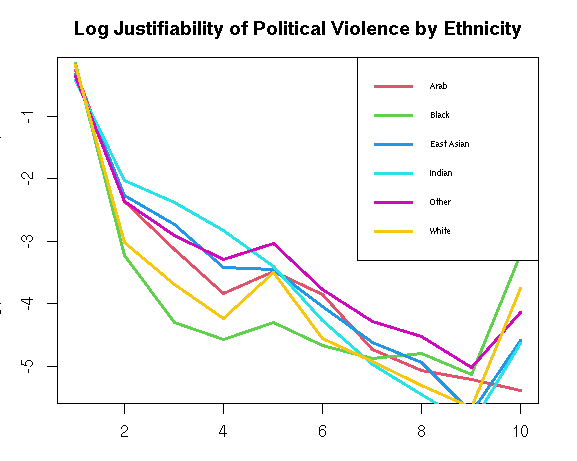
\includegraphics[scale=0.8]{ethterror.jpeg}

This is progress because we managed to get some fits that catch the tails.  However, this was totally a matter of trial and error and we do need to produce rigorous theoretically sound methods too.

Once again, progress in science took place with an anarchic messy ad hoc, intuitive, just as Paul Feyerabend had suspected about how science actually progresses.

\section{Example of a Successful Fit}

I won't worry about interpretation at the moment.  I will show you the data and two fits.  In the graph you will see data in 'X' and three lines.  One is a regression line on the entire data set.  For this $R^2=0.54$.  The other two are broken lines of two regression line fits; their individual goodness of fits are $R^2=0.7$ and $R^2=0.59$ which are both better than the single regression.  This is beautiful success.  The Log-V idea has yielded fruit.

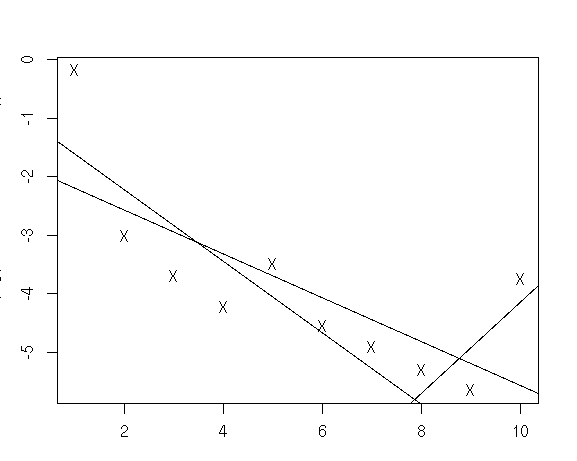
\includegraphics[scale=0.8]{logv.jpeg}

\section{Mixture of opposing exponentials}

We suppose that the population is driven by two factors, say $g_1,g_2$.  We don't care what they are yet, but they are different.  
Next suppose $q_1+q_2=1$ are two proportions where fraction $q_1$ is driven by factor $g_1$ and fraction $q_2$ by $g_2$.  Then we hypothesize some pole $z_2$ with the convention $z_1=0$.  The density ought to have form

\begin{equation}
p(x, \lambda_1,\lambda_2, z_2, q_1, q_2) = q_1 \lambda_1 e^{-\lambda_1 x} + q_2 \lambda_2 e^{-\lambda_2(z_2 - x)}
\end{equation}

This may seem a bit messy but it's just two opposing exponentials with mass fraction $(q_1, q_2)$ on each .  Our whole effort above is to find $(\lambda_1, \lambda_2, z_2, q_1,q_2)$

The interpretation is very simple.  What we have before is the aggregate of two distributions and our statistical procedure will separate the two latent groups and give us information about them.


\section{Synthetic Idea of Terror}

I think that tail end people say $t=9,10$ are actually aggregates of a longer scale.  This is a synthetic model idea.

\begin{verbatim}
> exp(-0.611*8)
[1] 0.00753648
> 0.611*8/0.7766
[1] 6.294102
> z2 <- 8 + 6.294

mixture<-function(x) q1*(-a1)*exp(a1*x)+q2*a2*exp(-a2*(z2-x))

\end{verbatim}

This is a synthetic graph where we have a scaled backward exponential whose pole is further to the right of $x=10$. 

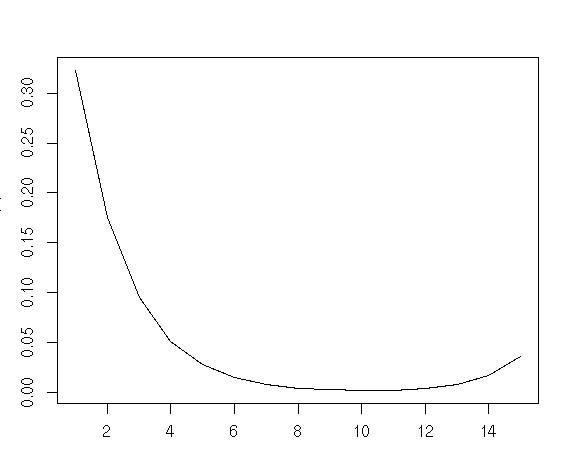
\includegraphics[scale=0.8]{synthterror.jpeg}

What is good about this expanded synthetic view is that $a_2$ is then properly interpreted as an exponential.  This then considers $x=10$ population to actually represent higher levels of propensity for violence aggregated and stretches it out to an appropriate distance to the right.

This approach does very little to the main mass of the left exponential and provides interpretability of the tail end mass in a parsimonious manner.

The graph of the density looks quite parsimonious and interpretable.  This is the idea behind a Rousseau-Hobbes decomposition of moral nature of Man.



 

\end{document}